\newpage
\section{DQN 算法}

使用一个参数化函数 $Q_\theta$ 拟合数据, 以此估计 $Q$. 

\subsection{CartPole 环境}
车杆环境. 状态值是连续的, 动作是离散的. 

\begin{figure}[!htb]
    \centering
    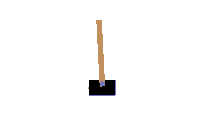
\includegraphics[width=0.618\linewidth]{pic/RL7/CartPole 环境}
    \caption{CartPole 环境}
\end{figure}


车杆环境中, 有辆车, 智能体的任务就是通过左右移动保持车上杆竖直, 若杆倾泻度数过大, 或者车子离初始位置偏离过大, 或坚持超过 200 帧, 则游戏结束. 智能体的状态是四维向量, 每一维都是连续的, 动作是离散的, 动作空间大小为 2. 每坚持一帧获得1分, 坚持 200 帧分最高. 

\begin{table}[!htb]
    \centering
    \caption{CartPole 环境状态空间与动作空间}
    \begin{tabular}[c]{ccc}\toprule
        意义 & 最小值 & 最大值 \\ \midrule
        车的位置 & $-2.4$ & $2.4$ \\
        车的速度 & $-\inf$ & $\inf$ \\
        杆的角度 & $\sim -24^\circ$ & $\sim 24^\circ$\\
        杆尖端的速度 & $-\inf$ & $\inf$ \\ \cmidrule{1-1}
        左移动小车 \\
        向右移动小车\\
        \bottomrule
    \end{tabular}
\end{table}

\subsection{DQN}

\begin{algorithm}[htb]
    \caption{DQN}
    \begin{algorithmic}
        \State 随机参数 $\omega$ 初始化 $Q_\omega(s,a)$
        \State 复制参数 $\omega^-\leftarrow \omega$ 初始化目标网络 $Q_{\omega^-}$
        \State 初始化经验回放缓冲区 $R$
        \For{序列 $e=1\to E$}
            \State 获取环境初始状态 $s_1$
            \For{时间步 $t=1\to T$}
                \State 以 $\epsilon-$greedy, 根据 $Q_\omega(s,a)$ 选择当前状态 $s_t$ 动作 $a_t$
                \State 得到环境反馈 $r_t, s_{t+1}$
                \State 将 $(s_t,a_t,r_t,s_{t+1})$ 放入缓冲区 $R$
                \If{$R$ 中数据足够}
                    \State 从 $R$ 采样 $N$ 个数据 $\{ (s_i,a_i,r_i,s_{i+1}) \}_{i=1,\dots,N}$
                    \State 对每个数据, 计算 $\displaystyle y_i=r_i+\gamma \max_a Q_{\omega^-}(s_{i+1}, a)$
                    \State 最小化目标损失 $\displaystyle L=\frac{1}{N}\sum_i \left[y_i - Q_\omega(s,a)\right]^2$
                    \State 更新当前网络 $Q_\omega$
                    \State 累积 $C$ 步后, 更新目标网络 $\omega^-\leftarrow \omega$
                \EndIf
            \EndFor
        \EndFor
    \end{algorithmic}
\end{algorithm}

使用神经网络拟合动作价值函数 $Q(s,a)$. 若动作是连续的, 网络输入 $s,a$, 输出一个标量, 表示在 $s$ 下采取 $a$ 的价值. 若动作是离散的, 除了输出价值的做法, 还可以仅输入 $s$, 输出每一个动作的 $Q$. 通常 DQN 以及 Q-learning 只能处理动作离散的情况, 因为 $Q$ 函数更新时用到了 $\max_a$ 的操作. 假设神经网络的参数是 $\omega$, 每个 $s$ 下 $a$ 的 $Q$ 表示为 $Q_\omega (s,a)$. 将此神经网络称为 $Q$ 网络. 

其目标应该和 Q-learning 目标 $r+\gamma \max_{a'\in\AC}Q(s',a')$ 靠近, 所以对于一组 $\{ (s_i, a_i, r_i, s'_i) \}$, $Q$ 网络损失函数可以构造为均方误差形式:
\begin{align*}
    \omega^* = \argmin_\omega \frac{1}{2N}\sum_{i=1}^N\left[ Q_\omega(s_i, a_i) - \left( r_i + \gamma \max_{a'} Q_\omega (s'_i, a') \right) \right]^2
\end{align*}

由于 DQN 是离线算法, 所以使用 $\epsilon-$greedy 策略平衡探索与利用. 但还有些 trick, 让其更加稳定与出色. 

\subsubsection{经验回放}
一般有监督学习中, 都假设训练数据是独立同分布的, 每个 epoch 从数据中随机采样若干个数据进行梯度下降, 随着 epoch 增多, 一个数据可能被用多次. 但 Q-learning 一个数据只会被用一次. 所以 DQN 采用了经验回放, 维护一个回放缓冲区, 每次从环境采样的 $(s,a,r,s')$ 存到缓冲区, 训练时从缓冲区采样. 这样有两个好处:
\begin{enumerate}
    \item 样本满足独立同分布假设. MDP 采样的数据本身是不满足独立同分布假设的, 这一时刻状态与上一时刻相关. 这会使神经网络过拟合到最近的训练数据上. 经验回放可以打破样本间的相关性, 抑制过拟合.
    \item 提高样本效率, 一个样本可以用多次. 
\end{enumerate}


\subsubsection{目标网络}
DQN 最终目标是让 $Q_\omega (s,a)$ 逼近 $r+\gamma \max_{a'\in\AC}Q(s',a')$. 但是由于这个误差包含神经网络的输出, 让训练十分不稳定. 于是 DQN 使用目标网络: 先将误差中的网络固定, 训几轮后再同步参数, 这需要用两个网络:
\begin{enumerate}
    \item 原始网络 $Q_\omega(s,a)$, 用于损失函数前一项.
    \item 目标网络 $Q_{\omega^-}$, 用于计算损失函数后一项. $\omega^-$ 表示其参数. 
\end{enumerate}
目标网络使用较久的参数, $Q_\omega(s,a)$ 每一步都会更新, 目标网络每隔 $C$ 步后, 参数才会与原始网络同步 $\omega^-\leftarrow \omega$. 让训练更稳定.





